\documentclass[12pt]{report}

\usepackage{thesis}
\usepackage{minted}

\usepackage{nomencl}
\makenomenclature
% Set line spacing for the nomenclature entries
\setlength{\nomitemsep}{-\parsep}
% Nomenclature group titles
\renewcommand{\nomgroup}[1]{
  \ifthenelse{\equal{#1}{Q}}{
    \item[\large\textbf{\textsf{Quaternion}}]
  }{
    \ifthenelse{\equal{#1}{B}}{
      \item[\large\textbf{\textsf{Body Rate}}]
    }{
      \ifthenelse{\equal{#1}{M}}{
        \item[\large\textbf{\textsf{Matrix Algebra}}]
      }{
        \ifthenelse{\equal{#1}{C}}{
          \item[\large\textbf{\textsf{Computer Science}}]
        }{
          \item[\large\textbf{\textsf{Other}}]
        }
      }
    }
  }
}


% TODO Items
\newcommand\TODO[1]{\textcolor{red}{[TODO: #1]}}

\usepackage{comment}


\begin{document}

\renewcommand{\theFancyVerbLine}{
   \sffamily\textcolor[rgb]{0.5,0.5,0.5}{\scriptsize\arabic{FancyVerbLine}}}


\pagenumbering{roman}

\thesistitle
{DEVELOPMENT OF A HIGH-INTEGRITY ANALYTICAL AND EXPERIMENTAL TESTBED FOR OBSERVER-BASED CONTROLLERS FOR NASA's MAGNETOSPHERIC MULTISCALE MISSION SPACECRAFT}
{Daniel R. Couture}
{B.S., University of New Hampshire, 2001}
{Master of Science\\in\\Mechanical Engineering}
{May, 2014}
{2014}



\thispagestyle{empty}
\noindent This thesis has been examined and approved.
\vspace*{2.5cm}

\begin{minipage}{0.2\textwidth}
        \begin{flushleft}
        \end{flushleft}
    \end{minipage}
\begin{minipage}{0.8\textwidth}
        \begin{flushleft}
            \underline{\hspace{10cm}} \\
            Thesis Director, Dr. May-Win L. Thein\\
            Associate Professor of Mechanical Engineering\\
            \vspace{1.5cm}
            \underline{\hspace{10cm}} \\
            Dr. Barry Fussell\\
            Professor of Mechanical Engineering\\
            \vspace{1.5cm}
            \underline{\hspace{10cm}} \\
            \TODO{Find third professor}
            \vspace{2cm}
            \hspace{3cm}\underline{\hspace{7cm}} \\
            \hspace{3cm}Date
        \end{flushleft}
\end{minipage}\\[1cm]

\pagebreak

\linespread{1}

\addcontentsline{toc}{chapter}{Acknowledgements}
\begin{center}
\textbf{\large Acknowledgements}
\end{center}


I would like to fin ack

%\chapter*{Acknowledgements}
%\addcontentsline{toc}{chapter}{Acknowledgements}
%\label{chap:acknowledgements}


\pagebreak
\tableofcontents


\pagebreak
\addcontentsline{toc}{chapter}{List of Tables}
\label{chap:tables}
\listoftables


\pagebreak
\addcontentsline{toc}{chapter}{List of Figures}
\label{chap:figues}
\listoffigures

\pagebreak
\addcontentsline{toc}{chapter}{Nomenclature}


\nomenclature[Q]{$\bs{q_n}$}{nutation quaternion}
\nomenclature[Q]{$\bs{q}$}{quaternion where $\bs{q} = q_1\bs{i}+q_2\bs{j}+q_3\bs{k}+q_0$}
\nomenclature[Q]{$\bs{q_k}$}{quaternion state at discrete step $k$}
\nomenclature[Q]{$\bs{q_r}$}{rotational quaternion}
\nomenclature[Q]{$\bs{q_I}$}{identity quaternion where $\bs{q_I} = 0\bs{i}+0\bs{j}+0\bs{k}+1$}
\nomenclature[M]{$\bs{\Omega}$}{skew symmetric matrix}
\nomenclature[B]{$\bs{\omega}$}{Body Rate}

\printnomenclature


% \begin{tabular}{|l|c|c|}
%   \hline
%   % after \\: \hline or \cline{col1-col2} \cline{col3-col4} ...
%  \T \B \bf{Variable Name} & \bf{Symbol} & \bf{Units} \\ \hline
%  \T \B   Full quaternion & $\bf{\bar{q}}$ & -  \\ \hline
%  \T \B Quaternion imaginary vector & $\bf{q}$ & -  \\ \hline
%  \T \B Quaternion scalar component & $\bf{q_0}$ & -  \\ \hline
%  \T \B Spacecraft angular rates & $\boldsymbol{\omega}$ & $rad/s$  \\ \hline
%  \T \B Time derivative of full quaternion & $\bf{\dot{\bar{q}}}$ & -   \\ \hline
%  \T \B Time derivative of spacecraft angular rates & $\boldsymbol{\dot{\omega}}$ & $rad/s^2$   \\ \hline
% \multirow{2}{*} \T \B Angular rate augmented with zero for quaternion& $\boldsymbol{\bar{\omega}_{b/o}}$ & $rad/s^2$   \\
%      operators  & &  \\  \hline
% % \T \B Acceleration at expected location of accelerometer & $\bf{a}_{nom}$ & $m/s^2$  \\ \hline
%  \T \B True acceleration at location of accelerometer & $\boldsymbol{a}_{true}$ &  $m/s^2$   \\ \hline
% \multirow{2}{*} \T \B Acceleration where accelerometer is thought  & {$\boldsymbol{a_{nom}}$} &  $m/s^2$ \\
%     to be and oriented & & \\ \hline
%  \T \B Measured acceleration ($a_{true}$ + noise) & $\boldsymbol{a_m}$ & $m/s^2$  \\ \hline
% \multirow{2}{*} \T \B Acceleration at true accelerometer location,  & $\boldsymbol{a_{shift}}$ & $m/s^2$  \\
%    aligned to body axis & & \\ \hline
% \multirow{2}{*} \T \B Acceleration at true accelerometer location, & $\boldsymbol{a_{mis}}$ & $m/s^2$  \\
%      aligned to accelerometer axis & & \\ \hline
%  \T \B Accelerometer sensor bias & $\boldsymbol{a_b}$ & $m/s^2$  \\ \hline
% \multirow{2}{*} \T \B Shift in accelerometer location from measured & $\boldsymbol{\delta r}$  & $m$  \\
%    location   & &  \\ \hline
% \multirow{2}{*} \T \B accelerometer axes orthogonal rotation defined & $\boldsymbol{\delta}$  & $rad$  \\
%     by a small angle 1-2-3 Euler angle sequence & & \\ \hline
% \multirow{2}{*} \T \B Rotation matrix defining accelerometer axes  & $\boldsymbol{\Delta}$  & -  \\
%     orthogonal rotation & & \\  \hline
%  \T \B Lumped bias correction term & $\boldsymbol{a}_{LB}$  & $m/s^2$  \\ \hline
%  \T \B Spacecraft true inertia tensor & $\boldsymbol{J}$ & $kg-m^2$  \\ \hline
%  \T \B Nominal (model) spacecraft inertia tensor & $\boldsymbol{\hat{J}}$ & $kg-m^2$  \\ \hline
%  \T \B Measured accelerometer location prior to launch &  $\boldsymbol{r}$ & $m$  \\ \hline
%  \T \B Accelerometer white noise & $\boldsymbol{\nu}_{accelerometer}$ & $m/s^2$  \\ \hline
%  \T \B Torques on spacecraft & $\boldsymbol{T}$ & $N-m$  \\ \hline
%  \T \B State covariance matrix & $\boldsymbol{Q}$ & -  \\ \hline
%  \T \B Sensor noise covariance matrix & $\boldsymbol{R}$ & - \\ \hline

%   \hline
% \end{tabular}



%\section{Nomenclature}
%\begin{description}
%  \item[$\bf{\bar{q}}$] Full quaternion
%  \item[$\bf{q}$] Quaternion imaginary vector
%  \item[$\bf{q_0}$] Quaternion scalar component
%  \item[$\boldsymbol{\omega}$] Spacecraft angular rates
%  \item[$\bf{\dot{\bar{q}}}$] Time derivative of full quaternion
%  \item[$\boldsymbol{\dot{\omega}}$] Time derivative of spacecraft angular rates
%  \item[$\boldsymbol{\bar{\omega}_{b/o}}$] Angular rate augmented with zero for quaternion operators
%  \item[$\boldsymbol{a_{true}}$] True acceleration at location of accelerometer
%  \item[$\boldsymbol{a_{typ}}$] Acceleration where accelerometer is thought to be and oriented
%  \item[$\boldsymbol{a_m}$] Measured acceleration ($a_{true}$ + noise)
%  \item[$\boldsymbol{a_{shift}}$] Acceleration at true accelerometer location, aligned to body axis
%  \item[$\boldsymbol{a_{mis}}$] Acceleration at true accelerometer location, aligned to accelerometer axis
%  \item[$\boldsymbol{a_b}$] Accelerometer sensor bias
%  \item[$\boldsymbol{\delta r}$] Shift in accelerometer location from measured location
%  \item[$\boldsymbol{\delta}$] 1-2-3 small angle Euler rotation defining accelerometer axes orthogonal rotation
%  \item[$\Delta$] Rotation matrix defining accelerometer axes orthogonal rotation
%  \item[$a_{LB}$] Lumped bias correction term
%  \item[$J$] Spacecraft inertia tensor
%  \item[$\hat{J}$] Expected spacecraft inertia tensor
%  \item[$r$] Measured accelerometer location prior to launch
%  \item[$\nu_{accelerometer}$] Accelerometer white noise
%  \item[$T$] Torques on spacecraft
%  \item[$Q$] State covariance matrix
%  \item[$R$] Sensor noise covariance matrix
%\end{description}


\pagebreak

\begin{abstractpage}
\TODO{Pull highlight from completed thesis}

\end{abstractpage}

% This thesis presents several methods for the on-board and/or ground-based calibration of accelerometers for the spacecraft (s/c) of the NASA Magnetospheric MultiScale (MMS) Mission during mission operation. A lumped bias is estimated to correct for the total effect of the MMS accelerometer sensor bias, orthogonal misalignment and the shift in the s/c's center of mass.

% Various estimation techniques are evaluated and compared, including both dynamically driven real-time filters/observers and post processing batch algorithms. Both methods are shown to accurately determine lumped bias, so long as the s/c inertia tensor is well known. If, however, there is any uncertainty in the inertia tensor, only post processing methods yield accurate lumped bias estimates. Analytical simulations show that these methods are able to correct accelerometer readings to within 1 micro-g of true acceleration. Preliminary experimental verification also shows proof of concept.



%%%%% ^^ 136 words currently (14 more allowable)
%
%This thesis will present multiple (methods) for the calibration of the accelerometers used on-board NASA's MMS spacecrafts. A lumped bias will be estimated to (simultaneously) account for the accelerometer's sensor bias, orthogonal misalignment as well as a shift in the spacecraft's center of mass. The lumped bias will be shown to effectively correct for all unknown parameters to within 1 micro-g of the true (state/acceleration).
%
% Various methods will be (compared/evaluated) and both dynamically driven real-time filters as well as post-processing batch algorithms will be shown to successfully determine the lumped bias if the inertia tensor is known accurately. If there is error in the (estimated/measured) inertia tensor, however only the post processing method yielded an (accurate) lumped bias (term/vector).

%No more than 150 words, no tables, no figures, no symbols now sub/superscripts or greek letter.


%what it is
%what its for/why
%what the research will show



\pagenumbering{arabic}

\chapter{Background}
\label{chap:Background}

The National Aeronautics and Space Administration (NASA) is planning to launch the Magnetospheric Multiscale (MMS) Mission into orbit around the Earth in order to study reconnection of the magnetic fields.  The effects of the phenomenon can be clearly seen in disturbances to spacecraft, GPS signals, and even inducing current in the power grid to the point of causing outages.  Although the effects are readily observed the internal dynamics and modeling is only theorized.  The causes of magnetic field reconnection trace back to coronal mass ejections (CME) from the sun.  These CMEs contain their own magnetic field properties that on collision with the Earth's fields can cause opposing field lines to cross and then separate.  This crossing and separation is called reconnection.  Its occurrences can open up portals allowing plasma from the interstellar medium to connect with plasma of the Earth's magnetosphere and produce a release of a large amount of energy.  A reconnection event starts on the dayside magnetopause of the Earth and
rapidly folds over to magnetotail.  The diffusion region of the event can travel at about \TODO{lookup speed} and has a thickness of \TODO{lookup thickness} which can pass orbiting satellites in a fraction of a second.  Theories about the internal structure of the diffusion region \TODO{reference active theories} have been difficult to test because of the speed of the event.  The general approach to getting a full view of the area surrounding a satellite is to mount a sensor facing out from the satellite and set the satellite to be spin stabilized so that through the turn a series of observations can be made and then stitched together to form a full field of view.  In order for this approach to be partially successful the satellite would have to be spinning at about 600 rpm to get a single full view image, which for a moderate sized satellite would introduce a restrictive amount of rotational dynamics coumpounded by the fact that each MMS satellite has 4 Spin-plane Double Probe (SDP) booms \TODO{work in
reference to UNH R. B. Torbert for FIELDS investigation} extending about 50 meters out from the spacecraft (s/c) body and two Axial Double Probe (ADP) booms extending 10 meters out along the rotational axis.  The potential 600 rpm speed would translate into a SDP tip velocity around 3,000 meters per second.
The approach taken by the MMS team is to mount a series of instruments around the s/c to have a full view at all times.  This in conjunction with the rate of measurements each instrument can take will provide a much richer set of data for the mission scientists to analyze.


\chapter{System State Representation}
\label{chap:SystemStateRepresentation}

Should this section be part of the Estimators section or just prior to??

Talk about quaternions in here, and define quaternion multiplication, how quaternions are adjusted.  Conversion between body rates and changes in quaternions.  Reference differences in rotation and nutation quaternion measurements and link to their use in the controller's section of the thesis.



\chapter{Code Versions}
\label{chap:CodeVersions}

\section{Control Loop in Simulink}
\label{sec:ControlLoopinSimulink}





\chapter{TSatPy}
\label{chap:TSatPy}

Chapter \ref{chap:ProgressionOfControlSystemSoftware} detailed the progression through the initial four versions of the attitude determination and control system (ADCS) that are written in or for a Numerical Simulation Software (NSS) implementation.  While these versions provide a level of insight and control into a control system, the NSS environment is not a natural fit for that level of programming and presents issues that take a significant effort to work around.  On top of some of the issues with diagnosing problems, the NSS controller code targets a fairly narrow swath of professions that are comfortable with using and editing it.  Because of this, the final version was written in Python, a common cross-platform and open source programming language.

Python is quoted as coming ``batteries included'' which is a statement to the number of common libraries that come standard with the language including a \verb|socket| library for sending and receiving User Datagram Protocol (UDP) packets used by TableSat.  Python is also known as an expressive language where what a section of code does is generally easily discernible from a quick read.

To support the control system written for this thesis being easily available for others to use and edit, python includes a variety of unit test frameworks for ensuring consistency, and gives the ability to write self-documenting code.  Self-documenting code means that if have an instance of a class stored in a variable \verb|v| but are unsure what can be done with the class, typing \verb|help(v)| will print out documentation about the various methods available and how they are used.

Section (\ref{sec:KeyCharacteristics}) covers some of the notable characteristics about the TSatPy implementation of the ADCS, and Section (\ref{sec:Module Design}) describes the different types of classes that are written for the program and what their role is.

\section{Key Characteristics}
\label{sec:KeyCharacteristics}

\subsection{Adaptive Step Algorithms}

All time dependent calculations vary their parameters at run-time dependent on the time since the last time it ran. For example, the integral component of a PID controller with an error measure of $+0.2$ will accumulate an error of $+0.02$ for the first $\Delta t_k = 0.1$ sec, but will only accumulate an additional $+0.016$ for the next time step of $\Delta t_{k+1} = 0.08$ sec.  This functionality avoids the errors encountered when a system is linearized about an assumed time step, but the actual time step varies which causes the controller gain values to be over or under aggressive.

\subsection{Variable System Clock}

The system clock is the official time keeper for the entire ADCS. Advantages to using a central clock instead of the computer time is that the rate of elapsed time can be modified at run-time during simulations to either compress the time to complete the simulation or slow down the simulation to inspect a transient event. (See Section \ref{subsec:IntegralEstimator})

\subsection{Quaternion Multiplicative Corrections}

Quaternions that quantify a system's position contain 4 values that through common control systems implementations are tracked and controlled separately. This approach ignores the restriction that rotational quaternions maintain a unit norm while the adjustments are made then scale the resulting quaternion back to a unit norm compromising the predictability and stability of the control system.  Using the object oriented programming to track the scalar and vector components ensures that controllers can be built that make use of the quaternion multiplicative correction technique which maintains the integrity of the values and their relation to the physical attitude of the system. (See Section \ref{subsec:QuaternionAttitude})

\subsection{Theta Multiplier with Quaternion Vector Balancing}

Unlike body rates that can be linearly scaled, the 4 quaternion values are sinusoidal values where multiple values can represent the same attitude (i.e. 0, 360 degrees). Scaling the sinusoidal values directly produces inconsistent adjustment rates. All quaternion scaling in the TSatPy software is performed against angle that the quaternion represents. With this method, we can maintain the linear scaling affect that is desired while maintaining the integrity of the quaternion representation. (See Section \ref{subsec:ThetaMultiplierWithQuaternionVectorBalancing})

\subsection{Run-time interface}

Through the use of a python twisted daemon process an restful API interface is available to query the state of the system in the middle of a run. This creates the ability to display meaningful representations of the system and increase insight into the system's dynamic behavior instead of relying on batch post processing.  This functionality is built into the last NSS version of the software, but has not yet been ported over to the python code base. (See Section \ref{sec:ObjectOrientedNSSControlSystem})

\subsection{Concurrent Estimation/Control Algorithms}

When running a comparative analysis between different types of estimators or different types of controllers, common methods are to re-run simulations for each variation and compare the results. The library allows for configurations such as providing the same measurement values to both a PID and SMO estimator to compare their performance. (See Section \ref{sec:ComparativeAnalysysofPIDandSMOEstimators})

\subsection{Quaternion Decomposition}

With spin-stabilized satellites, five degrees of freedom are available to compare against a fixed desired value.  The quaternion decomposition method allows the separation of the yaw motion from the remained of the attitude representation enabling the 5-DOF control of constant body rates and removing nutation. (See Section \ref{subsec:SpinStabilizedControl})

\subsection{Modular Design}

This library is designed to have interchangeable components with predefined and consistent interfaces and roles by allowing for the inclusion of additional estimation and control techniques. In the case of estimation, an Extended Kalman Filter (EKF) class can be added by creating a new class in Estimator.py that has contains the common properties ($\bs{\hat{x}}$, $\bs{x}_e$..) and common methods ($\bs{\hat{x}}$ = update($\bs{x}$)).

\subsection{Portable Design}

The portable design dictates that with the defined interfaces between modules, the observer based control methods have no knowledge of what is producing the sensor readings and what is accepting moment commands. This enforces consistency in the behavior of the system whether it's hooked up to an in-memory model of a satellite, NASA MMS TableSat 1A, or any future spin spin-stabilized platform.

\subsection{Python}

There can be a disconnect between the control systems engineer that regularly complete their design and analytical work in a Numerical Simulation Software environment (like Matlab Simulink or Octave) and the software engineer who implementation the control method in a more standard language. By using a language like python, the code can be written in an expressive manner so that a control systems professional only needs a little programming experience to modify the code. It also keeps the controller in a language than could be reviewed for optimization by a software engineer and applied directly to the experimental platform without requiring a conversion to an entirely different system or language.


\section{Module Design}
\label{sec:Module Design}

Below is an outline of the separate modules contained in the TSatPy library and their associated roles.

\subsection{Actuators}
\label{subsec:actuators}

input: Desired moment\\
output: Actual moment\\

This module defines the output of the controller. The actuator instance on initialization, is supplied with the physical arrangement of the actuators. During run-time the actuator module first accept a $\Re^3$ moment from the controller.  It then compares what it's being asked to do with what can actually be supplied.  That true moment is then available for use with estimator state propagation, and for conversion to actuator voltages. (See Section \ref{sec:ActuatorConfiguration})

\subsection{ADCS}
\label{subsec:ADCS}

input: Configuration file\\
output: ADCS model\\

This module is intended as the main parent object.  As an input it will read a json configuration file that defines all the components and parameters required for a specific observer-based controller.


\subsection{Clock}
\label{subsec:Clock}

input: None\\
output: Elapsed time\\

This module establishes the authoritative source for elapsed time and is continually referenced by any time-dependent logic such as integral or derivative based parameters. The metronome class by default track seconds since the initialization of the clock, but when running simulations can have it's speed dynamically altered to either run faster for long term simulations or run slower to get better inspection of an event.


\subsection{Comm}
\label{subsec:Comm}

From Controller to Satellite\\
input: Voltage setting determined by the actuator\\
output: UDP packet to the system or in-memory model\\
From Satellite to Controller\\
input: Sensor voltages from the system or in-memory model\\
output: Sensor data to submit to sensor class for conversion to a state\\

This module handles the interface between the the control system and either the physical system or the theoretical model. With the physical system, a UDP socket is opened and either listens for packets transmitted from the sensors or submits voltage packets to set actuator voltages. When running in simulations, the module submits and receives the voltage messages to an in-memory model of the system that contains the system dynamics and can return mocked sensor voltages based on the behavior.


\subsection{Controller}
\label{subsec:Controller}

input: Estimated state ($\bs{\hat{x}}$)\\
output: Moment couples ($\bs{M}$)\\

This module contains the algorithms that compare the estimated system behavior with the desired behavior and determine what moments required to make the system behave as desired.

The master controller instance governs the interface between the incoming estimator state and the outgoing actuator moments. The master controller can run multiple control algorithms simultaneously which can be individually tuned to different types of system behaviors like one that can handle large errors and one for the soft corrections at steady state.


\subsection{Estimator}
\label{subsec:Estimator}

input: Measured state ($\bs{x}$)\\
output: Estimated state ($\bs{\hat{x}}$)\\

This module contains the algorithm that take the measured state from the sensor model which is likely based on noisy sensor data and attempts to attenuate the effects of the noise to create an accurate representation of the true state of the system.

\subsection{Sensor}
\label{subsec:Sensor}

input: Voltages ($\bs{V}$)\\
output: Measured state ($\bs{x}$)\\

This module receives raw voltage measurements from either a simulated truth model of the system or from the Comm module polling sensor voltage data off the experimental TableSat.  Each class represents a different sensor type (coarse sun sensor, magnetometer, gyroscope, ...) and contain the logic to convert sensor readings from that sensor into a state representation $x$ with quaternion and body rates.


\subsection{Service}
\label{subsec:Service}

input: Run configuration\\
output: Twisted daemon\\

Coupled with the ADCS module the Service module is intended to create the daemon that manages the interactions between all the modules including sockets to TableSat.


\subsection{StateOperator}
\label{subsec:StateOperator}

input: An instance from the State module\\
output: A modified State instance or the conversion to a new State instance\\

This module contains classes that are designed to modify instances from the State module such as \verb|BodyRate| or \verb|Quaternion| or convert between them. For example an error quaternion can be scaled up or down by the QuaternionGain class.

\begin{table}[H]
  \centering
  \begin{tabular}{l|p{0.5\linewidth}}
    Class &  What it does \\ \hline
    BodyRateGain & Scale a BodyRate instance\\
    QuaternionGain & Scale a Quaternion instance\\
    StateGain &  Scale the State instance (Wrapper for QuaternionGain, BodyRateGain)\\
    QuaternionSaturation & Saturate a Quaternion\\
    BodyRateSaturation & Saturate a BodyRate\\
    StateSaturation  & Saturate a State (Wrapper for QuaternionSaturation, BodyRateSaturation)\\
    BodyRateToMoment & Convert a BodyRate to a Moment\\
    QuaternionToMoment & Convert a Quaternion to a Moment\\
    StateToMoment  & Convert a State to a Moment (Wrapper for QuaternionToMoment, BodyRateToMoment)\\
  \end{tabular}
  \caption{State Operators}
  \label{tbl:StateOperators}
\end{table}



\subsection{State}
\label{subsec:State}

This module contains classes that are used to quantify the state of the system.

\begin{table}[H]
  \centering
  \begin{tabular}{l|p{0.5\linewidth}}
State  & Class \\ \hline
Quaternion & Attitude \\
BodyRate & Body-fixed angular velocities \\
QuaternionError & Difference in attitudes \\
QuaternionDynamics & How body rates change the attitude \\
EulerMomentEquations & How moments change the body rates  \\
State & Position and velocity \\
StateError & Differences in position and velocity \\
Plant & In-memory model of the satellite \\
Moment & Applied torques \\
  \end{tabular}
  \caption{State Measurements}
  \label{tbl:State}
\end{table}



\chapter{TSatPy SOURCE CODE}
\label{chap:tsatpy_source}

\linespread{1}

\pagebreak
\section*{TSatPy/ADCS.py}\label{code:TSatPy/ADCS.py}\inputminted[linenos,fontsize=\scriptsize]{python}{/home/dcouture/git/mathyourlife/TSatPy/TSatPy/ADCS.py}

\pagebreak
\section*{TSatPy/Actuator.py}\label{code:TSatPy/Actuator.py}\inputminted[linenos,fontsize=\scriptsize]{python}{/home/dcouture/git/mathyourlife/TSatPy/TSatPy/Actuator.py}

\pagebreak
\section*{TSatPy/Clock.py}\label{code:TSatPy/Clock.py}\inputminted[linenos,fontsize=\scriptsize]{python}{/home/dcouture/git/mathyourlife/TSatPy/TSatPy/Clock.py}

\pagebreak
\section*{TSatPy/Comm.py}\label{code:TSatPy/Comm.py}\inputminted[linenos,fontsize=\scriptsize]{python}{/home/dcouture/git/mathyourlife/TSatPy/TSatPy/Comm.py}

\pagebreak
\section*{TSatPy/Controller.py}\label{code:TSatPy/Controller.py}\inputminted[linenos,fontsize=\scriptsize]{python}{/home/dcouture/git/mathyourlife/TSatPy/TSatPy/Controller.py}

\pagebreak
\section*{TSatPy/Estimator.py}\label{code:TSatPy/Estimator.py}\inputminted[linenos,fontsize=\scriptsize]{python}{/home/dcouture/git/mathyourlife/TSatPy/TSatPy/Estimator.py}

\pagebreak
\section*{TSatPy/Sensor.py}\label{code:TSatPy/Sensor.py}\inputminted[linenos,fontsize=\scriptsize]{python}{/home/dcouture/git/mathyourlife/TSatPy/TSatPy/Sensor.py}

\pagebreak
\section*{TSatPy/Server.py}\label{code:TSatPy/Server.py}\inputminted[linenos,fontsize=\scriptsize]{python}{/home/dcouture/git/mathyourlife/TSatPy/TSatPy/Server.py}

\pagebreak
\section*{TSatPy/Service.py}\label{code:TSatPy/Service.py}\inputminted[linenos,fontsize=\scriptsize]{python}{/home/dcouture/git/mathyourlife/TSatPy/TSatPy/Service.py}

\pagebreak
\section*{TSatPy/State.py}\label{code:TSatPy/State.py}\inputminted[linenos,fontsize=\scriptsize]{python}{/home/dcouture/git/mathyourlife/TSatPy/TSatPy/State.py}

\pagebreak
\section*{TSatPy/StateOperator.py}\label{code:TSatPy/StateOperator.py}\inputminted[linenos,fontsize=\scriptsize]{python}{/home/dcouture/git/mathyourlife/TSatPy/TSatPy/StateOperator.py}

\pagebreak
\section*{TSatPy/\_\_init\_\_.py}\label{code:TSatPy/__init__.py}\inputminted[linenos,fontsize=\scriptsize]{python}{/home/dcouture/git/mathyourlife/TSatPy/TSatPy/__init__.py}

\pagebreak
\section*{TSatPy/tests/Clock\_test.py}\label{code:TSatPy/tests/Clock_test.py}
\inputminted[linenos,fontsize=\scriptsize]{python}{/home/dcouture/git/mathyourlife/TSatPy/TSatPy/tests/Clock_test.py}

\pagebreak
\section*{TSatPy/tests/Controller\_test.py}\label{code:TSatPy/tests/Controller_test.py}
\inputminted[linenos,fontsize=\scriptsize]{python}{/home/dcouture/git/mathyourlife/TSatPy/TSatPy/tests/Controller_test.py}

\pagebreak
\section*{TSatPy/tests/Estimator\_test.py}\label{code:TSatPy/tests/Estimator_test.py}
\inputminted[linenos,fontsize=\scriptsize]{python}{/home/dcouture/git/mathyourlife/TSatPy/TSatPy/tests/Estimator_test.py}

\pagebreak
\section*{TSatPy/tests/Sensor\_test.py}\label{code:TSatPy/tests/Sensor_test.py}
\inputminted[linenos,fontsize=\scriptsize]{python}{/home/dcouture/git/mathyourlife/TSatPy/TSatPy/tests/Sensor_test.py}

\pagebreak
\section*{TSatPy/tests/StateOperator\_test.py}\label{code:TSatPy/tests/StateOperator_test.py}
\inputminted[linenos,fontsize=\scriptsize]{python}{/home/dcouture/git/mathyourlife/TSatPy/TSatPy/tests/StateOperator_test.py}

\pagebreak
\section*{TSatPy/tests/State\_test.py}\label{code:TSatPy/tests/State_test.py}
\inputminted[linenos,fontsize=\scriptsize]{python}{/home/dcouture/git/mathyourlife/TSatPy/TSatPy/tests/State_test.py}

\pagebreak
\section*{TSatPy/tests/\_\_init\_\_.py}\label{code:TSatPy/tests/__init__.py}
\inputminted[linenos,fontsize=\scriptsize]{python}{/home/dcouture/git/mathyourlife/TSatPy/TSatPy/tests/__init__.py}




% \munfig{Credit: http://mms.gsfc.nasa.gov}{2d_field_lines}{pretty/2d_earth_mag_field_lines.png}{0.4}


% \section{What is it?}
% 4 identical satellites
% consallation formation flight
% magnetospheric multiscale mission MMS
% constructed in Goddard Space Flight Center
% classifies as a Solar Terrestrial probe mission

% \todo{image of MMS}

% \section{Mission}

% Science questions to answer \cite{mms_website}
%     What determines when reconnection starts and how fast it proceeds?
%     What is the structure of the diffusion region?
%     How do the plasmas and magnetic fields disconnect and reconnect in the diffusion regions?
%     What role do the electrons play in facilitating reconnection?
%     What is the role of turbulence in the reconnection process?
%     How does reconnection lead to the acceleration of particles to high energies?


% \todo{image of formation flight}
% study microphysics of
% 	magnetic reconnection
% 	energetic particle acceleration
% 	turbulence
% Launch Readiness Date (LRD): October 2014 \cite{mms_website}
% s/c MMS-1, MMS-2..MMS-4
% reconnection: Electromagnetic engergy from the sun interacts with Earth's magnetosphere ausing magneti field lines to cross and create a burst of energy \cite{nasa_edge_video_ne_at_mms}
% magnetic reconnection measured ions and electrons as boundary passes to create 3d model of it passing by
% Fast plasma investigation
% probing the electron diffusion region (EDR) (passes too rapidly to get an accurate view with current equipment small (1-10 km) and rapidly moving (10-100 km/s))
% adjacent magnetic fields generally have significaltly different orientations such that when they intersect, a large amount of energy is dispursed within a small region in the form of heat and kinetic energy.  The region = diffuision region
% explore magnetic reconnection
% dynamic regions of magnetosphere
% orbits planned to pass through the upstream and downstream magnetic reconnection sites
% 1) day side - solar wind field lines connection
% 2) down stream -
% 3) plasma travels down and causes the Arura
% through magnetospheric reconnection, portals allow energetic particles to traverse from outside to the interior of the magnetosphere
% predict when solar space weather within the magnetosphere and if they will affect orbiting satellites
% adverse space weather within the magnetosphere can negatively impace spacecraft system health GPS, induce disruptive current in electrical grids, communictaions, increased radiation exposure on trans-polar flights

% Difficult to understand
% magnetic boundary passes satellites quickly so has been hard to measure
% MMS has intsruments to capture measurements
% Instruments mounted on all sides of the
% 8 sensors 1/30th sec instead of

% October 2014, Atlas five launch \cite{nasa_edge_video}

% \section{Team}
% International partnership Japan/US/French

% Marshall space flight Alabama calibrate DIS

% \section{Payload}
% Octagonal design
% 3.5 meters wide and 1.2 meters high

% 1,250 kg

% Sensors
% 	star sensor -> attitude
% 	accelerometers -> $\Delta V$

% Fast Plasma Instrument (FPI) - controls
% 	16 Dual Electron spectrometer (DES) Goddary built
% 	16 Dual Ion Spectrometer (DIS) Japan *** built, hand delivered
% 	180 degree and +- 22degree measurement
% 	30 millisec measurement rate 100x faster than previous missions entire view of sky
% FPI
% 	despins data

% Instument Data processing Unit (IDPU) - brains of measurements
% 	collects, compresses, transmits requested measurement data
% 	configure while on mission

% booms
% 	eight deployable booms
% 	two 12.5m axial booms (electric field sensors)
% 	four 60m wire booms
% 	two 5m booms in spin plane for magnetometers
% rigid, wire, top/bottom booms
% important to keep consistent spin rate to get accurate estimates of boom location

% \todo{image of spectrometers}

% \section{Propulsion}

% types: solid propellents, bi propellents, electro propulsion, cold gas systems
% chose: mono-propellant blowdown - hydrozene power thrusters \cite{nasa_edge_video_propulsion}
% 3 rpm
% radial thrusters - spinning
% axial thrusters - prevent nutation

% concern:
% propulsion introduce distrubances

% 20 second pulses

% fuel limits by number of adjustments

% monitor fuel left - via pressure, temperature via ideal gas law

% determine performance characteristics of the thrusters prior to launch, exit velocity

% dry mass, wet mass -> time variant mass

% responsible for maintaining accurate formation flight with interspacecraft separation from 100s of km down to 10 km

% planned orbit adjustment about 1 / 2weeks

% critical to fly in tetrahedron to achieve 3d model

% Earth Moon system influence to target the desired location/time

% \section{performance requirements}

% $\pm 0.5$ deg attitude tollerance
% 1/10th of a second


% \chapter{The Quaternion}\label{ch:quaternion}
% \pagenumbering{arabic}

% The concept of a quaternion first appeared in 1843 by William Rowan Hamilton \cite{kuipers}.  The use of the quaternion is a extension on the rules governing the mathematics behind imaginary/complex numbers which have rank 2 to a hyer-complex number of rank 4.

% \section{Origin}\label{sec:quaternion_origin}

% Complex number interactions through multiplication where $1 = 1 + 0i$ and $i = 0 + 1i$ are

% \eqntable{Complex Number Multiplication Table}{complex_multiplication}{|c|c|c|}{ \hline
% 	\times & 1 &  i \\ \hline
% 	1      & 1 &  i \\ \hline
% 	i      & i & -1 \\ \hline
% }

% When expanding this concept to create the quaternion, Hamilton defined the four orthogonal unit quaternions as

% \subeqn{
% 	1 &= 1 + 0\bs{i} + 0\bs{j} + 0\bs{k} \\
% 	i &= 0 + 1\bs{i} + 0\bs{j} + 0\bs{k} \\
% 	j &= 0 + 0\bs{i} + 1\bs{j} + 0\bs{k} \\
% 	k &= 0 + 0\bs{i} + 0\bs{j} + 1\bs{k}
% }

% and the initial interactions between the orthogonal unit quaternions were $i^2 = j^2 = k^2 = ijk = -1$ \cite{kuipers}.  From Hamilton's identity, the complex number multiplication table can be expanded to quaternion multiplication in Table \ref{eqn:quaternion_multiplication}.  Quaternion products are read as $\text{row} \otimes \text{column}$.  Note that the quaternion product is not cummutative as $i \otimes j = k$ but $j \otimes i = -k$.

% \eqntable{Quaternion multiplication table}{quaternion_multiplication}{|c|c|c|c|c|}{ \hline
% 	\otimes & 1 &  i &  j &  k \\ \hline
% 	1       & 1 &  i &  j &  k \\ \hline
% 	i       & i & -1 &  k & -j \\ \hline
% 	j       & j & -k & -1 &  i \\ \hline
% 	k       & k &  j & -i & -1 \\ \hline
% }

% \section{Quaternion Properties}

% The quaternion notation to be used in this thesis follows the structure of 4-tuple in $\Re^4$ where the $q_0$ scalar term follows the $\Re^3$ vector $\bs{q_v}$.

% \eqn{
% 	\bs{q} = \bs{q_v} + q_0 = \qinline{q_1}{+q_2}{+q_1}{+q_0}
% }

% \subsection{Equality}

% Two quaternions are equal if all components are equal.  This is not to be confused with their use for rotational quaternions where different quaternions can represent the same attitude \todo{link to section}.

% \eqn{
% 	\bs{q} = \bs{p} \iff q_1 = p_1,  q_2 = p_2,  q_3 = p_3,  q_0 = p_0
% }

% \subsection{Sum and Difference}

% The sum and difference of two quaternions is the piecewise combination of their components.

% \eqn{
% 	\begin{array}{c}
% 		\bs{q} + \bs{p} = \qinline{(q_1+p_1)}{+(q_2+p_2)}{+(q_3+p_3)}{+(q_0+p_0)} \\
% 		\bs{q} - \bs{p} = \qinline{(q_1-p_1)}{+(q_2-p_2)}{+(q_3-p_3)}{+(q_0-p_0)}
% 	\end{array}
% }

% \subsection{Norm}

% The norm or magnitude of the quaternion is

% \lbleqn{quaternion_norm}{
% 	\left\| \bs{q} \right\| = \sqrt{\bs{q_v} \cdot \bs{q_v} + q_0^2} = \sqrt{q_1^2+q_2^2+q_3^2+q_0^2}
% }

% \subsection{Unit Quaternion}

% A unit quaternion is one that has a norm of 1 ($\left\| \bs{q} \right\| = 1$) and has been introduced in the preliminary coverage of the quaternion in chapter \ref{ch:quaternion}.  Chapter \ref{ch:rotations} will cover how to implement a unit quaternion for modelling rotations.

% \subsection{Conjugate}

% The quaternion conjugate is defined as

% \eqn{
% 	\bs{q}^* = -\bs{q_v} + q_0 = \qinline{-q_1}{-q_2}{-q_3}{+q_0}
% }

% \subsection{Inverse}

% The quaternion inverse is the value that when multiplied by the original quaternion will yield the identity quaternion of $\bs{q} = \qinline{0}{+0}{+0}{+1}$

% \lbleqn{quaternion_inverse}{
% 	\bs{q}^{-1} = \frac{\bs{q}*}{\left\| \bs{q} \right\|^2}
% }

% In the case of a unit quaternion where $\left\| \bs{q} \right\| = 1$, the quaternion inverse $\bs{q}^{-1}$ and conjugate $\bs{q}^*$ are equivalent.

% \subsection{Skew Symetric Cross Product Matrix}

% Useful for matrix manipulation of quaternions, the skew symetric cross product matrix is often used to create part of a transformation matrix based on the vector portion of a quaternion.

% \eqn{
% 	\Omega(\bs{q}) = \smatrix{
% 		0    & -q_3 &  q_2 \\
% 		q_3  &  0   & -q_1 \\
% 		-q_2 &  q_1 &    0
% 	}
% }

% \section{Quaternion Product}

% The attitude quaternion and angular body rates are the two quantities that make up the system state in this thesis.  As such, the use of quaternions and specifically the quaternion product plays a key role in the simulation performance and accuracy.  In chapter \ref{ch:rotations} the use of Euler angles and quaternions are compared with details on why the quaternion approach was chosen.  Before moving into rotation specific quaternions lets first investigate the general definition of the quaternion product.

% Let two quaternions $\bs{q_a}$ and $\bs{q_b}$ be defined as:
% \subeqn{
% 	\bs{q_a} &= \bs{q_{av}} + q_{a0} = \qinline{q_{a1}}{+q_{a2}}{+q_{a3}}{+q_{a0}}\\
% 	\bs{q_b} &= \bs{q_{bv}} + q_{b0} = \qinline{q_{b1}}{+q_{b2}}{+q_{b3}}{+q_{b0}}
% }

% The quaternion product of $\bs{q_a} \otimes \bs{q_b}$ is expressed as
% \lbleqn{quaternion_product}{
%   \bs{q_a} \otimes \bs{q_b}
%   =
%   \bs{q_{av}} q_{b0} + \bs{q_{bv}} q_{a0} + \bs{q_{av}} \times \bs{q_{bv}} + q_{a0} q_{b0} - \bs{q_{av}} \cdot \bs{q_{bv}}
% }

% Exansion of equation \ref{eqn:quaternion_product} yields two sets of expressions.  One group evaluates to scalar values in $\Re$ and the other evaluates to vectors in $\Re^3$.
% \subeqn{
% 	\bs{q_v} &=
% 		\smatrix{q_{a1}\\q_{a2}\\q_{a3}} q_{b0} + \smatrix{q_{b1}\\q_{b2}\\q_{b3}} q_{a0} + \smatrix{q_{a1}\\q_{a2}\\q_{a3}} \times \smatrix{q_{b1}\\q_{b2}\\q_{b3}} \\
% 	q_0 &= q_{a0} q_{b0} - \bs{q_{av}} \cdot \bs{q_{bv}}
% }

% Evaluating the dot and cross products
% \subeqn{
% 	\bs{q_v} &=
% 		\smatrix{q_{a1}\\q_{a2}\\q_{a3}} q_{b0} + \smatrix{q_{b1}\\q_{b2}\\q_{b3}} q_{a0} + \smatrix{q_{a2}q_{b3}-q_{a3}q_{b2} \\
% 			q_{a3}q_{b1}-q_{a1}q_{b3} \\
% 			q_{a1}q_{b2}-q_{a2}q_{b1}
% 		} \\
% 	q_0 &= q_{a0}q_{b0}-(q_{a1}q_{b1}+q_{a2}q_{b2}+q_{a3}q_{b3})
% }

% \subeqn{
% 	\bs{q_v} &=
% 		\smatrix{
% 			q_{a1}q_{b0}+q_{b1}q_{a0}+q_{a2}q_{b3}-q_{a3}q_{b2} \\
% 			q_{a2}q_{b0}+q_{b2}q_{a0}+q_{a3}q_{b1}-q_{a1}q_{b3} \\
% 			q_{a3}q_{b0}+q_{b3}q_{a0}+q_{a1}q_{b2}-q_{a2}q_{b1}
% 		} \\
% 	q_0 &= q_{a0}q_{b0}-q_{a1}q_{b1}-q_{a2}q_{b2}-q_{a3}q_{b3}
% }

% Combining equations and ordering by $q_b$ components
% \eqn{
% 	\smatrix{\bs{q_v} \\ q_0} =
% 		\smatrix{
% 			 q_{b1}q_{a0}-q_{a3}q_{b2}+q_{a2}q_{b3}+q_{a1}q_{b0} \\
% 			 q_{a3}q_{b1}+q_{b2}q_{a0}-q_{a1}q_{b3}+q_{a2}q_{b0} \\
% 			-q_{a2}q_{b1}+q_{a1}q_{b2}+q_{b3}q_{a0}+q_{a3}q_{b0} \\
% 			-q_{a1}q_{b1}-q_{a2}q_{b2}-q_{a3}q_{b3}+q_{a0}q_{b0}
% 		}
% }

% Factoring out the $q_{b}$ quaternion
% \eqn{
% 	\smatrix{\bs{q_v} \\ q_0} =
% 		\smatrix{
% 			 q_{a0} & -q_{a3} &  q_{a2} & q_{a1} \\
% 			 q_{a3} &  q_{a0} & -q_{a1} & q_{a2} \\
% 			-q_{a2} &  q_{a1} &  q_{a0} & q_{a3} \\
% 			-q_{a1} & -q_{a2} & -q_{a3} & q_{a0}
% 		}
% 		\smatrix{q_{b1}\\q_{b2}\\q_{b3}\\q_{b0}}
% }

% From here the square matrix can be broken into a combination of quternion vector and scalar components along with a skew symetric matrix to generate a matrix version of the quaternion multiplication equation \ref{eqn:quaternion_product}.
% \eqn{
% 	\smatrix{\bs{q_v} \\ q_0} =
% 		\smatrix{
% 			\bs{\Omega}(\bs{q_{av}}) + \bs{I} q_{a0} & \bs{q_{av}} \\
% 			\bs{q_{av}}^T & q_{a0}
% 		}
% 		\smatrix{\bs{q_{bv}}\\q_{b0}}
% }

% The advantage to this notation is that is much easier to run in a matlab or other scripting language, but its layout is specific to our definition of the matrix where the scalar value follows the vector.  There is not clear consensus from the boader community on whether the vector or scalar should come first.  This can cause large issues when implementing a system using a externally provided library since both implementations expect a 4x4 matrix, and combining the logic from the two systems would require either rewritting of systems or spending extra cycles on the interface between the two systems converting the matrices from a scalar first to a scalar last layout and vice versa.

% The object oriented nature of the code written for this thesis reduces or eliminates the confusion.  When an instance of a quaternion class is created, the vector and scalar values are set as separate parameters on the object regardless of order.  So when used in computation the $\Re^3$ and $\Re^1$ values can be referenced directly through the vector and scalar properties respectively.  Chapter \ref{ch:object_oriented} will cover the structure of the code developed for the thesis in greater detail.  The specific code that governs interactions between quaternions in the model is in section \ref{code:lib/@quaternion/quaternion.m}.


% \chapter{Rotations}\label{ch:rotations}

% This chapter will focus on the computations required in order to represent a rotating body.  Section \ref{sec:euler_rotations} will cover the mathematics behind the standard Euler angle representation followed by an common implementation issues.  Section \ref{sec:quaternion_rotations} will detail the use of the unit quaternion and it's advantages over Euler angles in software implementations.

% \section{Euler Angle Rotations}\label{sec:euler_rotations}

% A Euler angle rotation matrix that requires a specified combination of rotations such as the common 3-1-3 transformation. To convert between the reference X, Y, and Z axes to the body's x, y, and z axis using the 3-1-3 transformation with angles $\psi$, $\theta$, $\phi$ respectively


% \lbleqn{euler_matrices}{
% 	\delta = \smatrix{\cos \psi & \sin \psi & 0 \\ -\sin \psi & \cos \psi & 0 \\ 0 & 0 & 1 }
% 	\gamma = \smatrix{ 1 & 0 & 0 \\ 0 & \cos \theta & \sin \theta \\ 0 &  -\sin \theta & \cos \theta }
% 	\beta = \smatrix{\cos \phi & \sin \phi & 0 \\ -\sin \phi & \cos \phi & 0 \\ 0 & 0 & 1 }
% }

% \eqn{
% 	\smatrix{x \\ y \\ z} = \beta \cdot \gamma \cdot \delta \smatrix{X \\ Y \\ Z}
% }

% where $\beta \gamma \delta$ expands to:

% \lbleqn{euler_rotation_matrix}{
% \smatrix{
% \cos \phi \cos \psi - \sin \phi \cos \theta \sin \psi &
% \cos \phi \sin \psi + \sin \phi \cos \theta \cos \psi &
% \sin \phi \sin \theta \\

% -\sin \phi \cos \psi - \cos \phi \cos \theta \sin \psi &
% -\sin \phi \sin \psi + \cos \phi \cos \theta \cos \psi &
% \cos \phi \sin \theta \\

% \sin \theta \sin \psi & -\sin \theta \cos \psi & \cos \theta \\
% }
% }

% There are three main issues with this approach.  First is that it is not unique.  While the 3-1-3 rotation shown above is the most common, twelve valid permutations exists (1-2-3, 1-3-2, 2-1-3, 2-3-1, 3-1-2, 3-2-1, 1-2-1, 1-3-1, 2-1-2, 2-3-2, 3-1-3, and 3-2-3) \todo{cite}.  The second issues is in the evaluation of the equations.  Their large dependency on trigonometric functions $\sin$ and $\cos$ make them both computationally more complex and prone to numerical drift as each trigonometric evaluation is an approximation whose accuracy depends on the library in use.  In the rotation matrix \ref{eqn:euler_rotation_matrix}, 29 trigonometric evaluations are required.  The third is the lack of expressiveness of the rotation matrix.  It is very difficult to determine what type of a rotation the matrix represents through visual inspection.

% Other issues develop when implementing a Euler angle based attitude system.  Evaluation of the system's Euler rates has its own set of issues.

% \lbleqn{euler_rate}{
% 	\smatrix{\dot{\psi} \\ \dot{\theta} \\ \dot{\phi}} = \frac{1}{\sin \theta}
% \smatrix{
% 	\sin \phi & \cos \phi & 0 \\
% 	\cos \phi \sin \theta & -\sin \phi \sin \theta & 0 \\
% 	-\sin \phi  \cos \theta & -\cos \phi \cos \theta & \sin \theta
% }
% \smatrix{\omega_x \\ \omega_y \\ \omega_z }
% }

% While \ref{eqn:euler_rate} has fewer trigonometric evaluations that in \ref{eqn:euler_rotation_matrix}, they can still contribute to numerical drift over time.  The most troublesome situation is known as a Gimbal lock where the Euler angle values can result in a loss of of a degree of freedom.  From \ref{eqn:euler_matrices} if $\theta=0$, the matrix $\gamma$ evaluates to the identity matrix which reduces the equation to two degrees of freedom.

% \eqn{
% 	\gamma
% = \smatrix{ 1 & 0 & 0 \\ 0 & \cos \theta & \sin \theta \\ 0 &  -\sin \theta & \cos \theta }
% = \smatrix{ 1 & 0 & 0 \\ 0 & 1 & 0 \\ 0 &  0 & 1 }
% }

% The Gimbal lock's effect is most evident in the Euler rate equations \ref{eqn:euler_rate} where $\theta = 0$ results in both a rank reduction of the matrix from three to two as well as a scalar multiplier that approaches infinity.

% \eqn{
% 	\smatrix{\dot{\psi} \\ \dot{\theta} \\ \dot{\phi}} = \frac{1}{0}
% \smatrix{
% 	\sin \phi & \cos \phi & 0 \\
% 	0 & 0 & 0 \\
% 	-\sin \phi  & -\cos \phi & 0
% }
% \smatrix{\omega_x \\ \omega_y \\ \omega_z }
% }



% \section{Quaternion Rotation}\label{sec:quaternion_rotations}

% The following section will describe the method required to perform a rotation of a body using the unit quaternion.  The unit quaternion is used since a full quaternion has four parameters and a rotation can be described in three parameters, typically roll/pitch/yaw.  The additional restriction that rotational quaternions have a norm of one $\left\| \bs{q} \right\| = 1$ reduces the free parameters to three.

% \subsection{Definition of a Rotational Quaternion}

% For the general quaternion in $\Re^4$ compared to the Euler angle representation described in section \ref{sec:euler_rotations}, the quaternion value has an extra degree of freedom.  To remove a degree of freedom from the quaternion to allow it to accurately represent the rotation in three degrees of freedom while containing the the information for a three dimensional vector and an angle of rotation.

% Rotational quaternion is defined as
% \lbleqn{quaternion_rotation_def}{
% 	\bs{q} = \bs{q_v} + q_0 = \bs{\hat{v}} \sin (-\theta/2) + \cos (-\theta/2)
% }

% where $\ds \bs{\hat{v}} = \frac{\bs{u}}{\left\| \bs{u} \right\|}$ and $\bs{u} \in \Re^3$, such that $\bs{q}$ can be interpreted as a rotation of $\theta$ radians about the axis of rotation $\bs{u}$.  Rotational quaternions are generally defined with a $+\theta/2$, but as will be demonstrated in \ref{subsec:q_rotate_a_point}, the negative sign allow us to rotate the points around a fixed coordinate plane instead of rotating the axes.  Combining equation \ref{eqn:quaternion_rotation_def} with the quaternion norm \ref{eqn:quaternion_norm} gives
% \eqntabular{rl}{
% 	\left\| \bs{q} \right\| &= \sqrt{q_1^2+q_2^2+q_3^2+q_0^2} \\
% 	&= \bs{\hat{v}_i}^2 \sin^2 (-\theta/2) + \bs{\hat{v}_j}^2 \sin^2 (-\theta/2) + \bs{\hat{v}_k}^2 \sin^2 (-\theta/2) + \cos^2 (-\theta/2) \\
% 	&= (\bs{\hat{v}_i}^2 + \bs{\hat{v}_j}^2 + \bs{\hat{v}_k}^2) \sin^2 (-\theta/2) + \cos^2 (-\theta/2) \\
% 	&= \sin^2 (-\theta/2) + \cos^2 (-\theta/2) \\
% 	&= 1 \\
% }
% which makes any rotational quaternion a unit quaternion and keeps an aditional restriction to reduce the degrees of freedom down to three.

% While this definition resolves the issue of an extra degree of freedom, there is still the issue of multiple representations of the same attitude.  In table \ref{eqn:multiple_rotations_quaternion}, multiple rotations about axis $\bs{\hat{v}} = 0\bs{i} + 0\bs{j} + 1\bs{k}$ are converted to their quternion representation.
% \eqntable{Multiple Rotation Angles and their Quaternion}{multiple_rotations_quaternion}{|c|c|}{ \hline
% 	\theta & \bs{q}(\bs{\hat{v}}, \theta) \\ \hline
% 	\pi / 2 - 4 \pi & \qinline{0}{+0}{+\frac{1}{\sqrt{2}}}{+\frac{1}{\sqrt{2}}} \\ \hline
% 	\pi / 2 - 2 \pi & \qinline{0}{+0}{-\frac{1}{\sqrt{2}}}{-\frac{1}{\sqrt{2}}} \\ \hline
% 	\pi / 2         & \qinline{0}{+0}{+\frac{1}{\sqrt{2}}}{+\frac{1}{\sqrt{2}}} \\ \hline
% 	\pi / 2 + 2 \pi & \qinline{0}{+0}{-\frac{1}{\sqrt{2}}}{-\frac{1}{\sqrt{2}}} \\ \hline
% 	\pi / 2 + 4 \pi & \qinline{0}{+0}{+\frac{1}{\sqrt{2}}}{+\frac{1}{\sqrt{2}}} \\ \hline
% }

% As with \ref{sec:euler_rotations}, there are multiple quaternion values that can represent the same orientation.  In the case of the quaternion though there are two representations for the rotation rather than the twelve Euler angle combinations.  During the development of the estimator and controller code, this duplicate representation of the same attitude caused trouble for most linear controllers.  For a constant body rate the angle of rotation would continually increase.  In this case, linear controllers models would not be able to identify that an attitude resulted from a rotation of $9\pi$ radians is the same a desired attitude from resulted from a $1\pi$ radian rotation and the controller would attempt to unwind the rotations.  If the controller was updated to keep the attitude angle restricted to a range of $0 \leq \theta < 2\pi$, this would remove the duplicate angle issue but introduce a new issue when the rotation traverses the $0, 2\pi$ boundary.  An estimate rotation of $\delta$ radians compared
% against a measured value of $2\pi - \delta$ where $\delta \ll 2\pi$ would almost max out the control effort since the error of $(2\pi - \delta) - (\delta) \approx 2\pi$ radians instead of the actual error of $2\delta$ radians.

% \subsection{Rotating a Point Using Quaternions}\label{subsec:q_rotate_a_point}

% In order to use the quaternions to visualize the rotation of the TableSat, we'll start with the rotation of a single point.  The implementation of this method can be reviewed in quaternion class in section \ref{code:lib/@quaternion/quaternion.m}.  The operation of the class will be covered in chapter \ref{ch:object_oriented}.

% A 3x3 rotational matrix is required to perform a rotation of a point in $\Re^3$ based on a rotational quaternion as it was with the 3-1-3 Euler angle rotational matrix noted in equation \ref{eqn:euler_rotation_matrix}.  The quternion based rotational matrix is created through
% \lbleqn{quaternion_rotation_matrix}{
% 	\bs{R_q} = (q_0^2 - \bs{q_v}^T\bs{q_v}) \bs{I} + 2 \bs{q_v} \bs{q_v}^T - 2 q_0 \bs{\Omega}(\bs{q_v})
% }


% To demonstate the usage of the $-\theta$ in equation \ref{eqn:quaternion_rotation_def}, the following example will rotate a point $A = (2, 4, -1)$ by $\pi/2$ radians about $\bs{\hat{v}} = 0\bs{i}+0\bs{j}+1\bs{k}$.  Substituting the rotation axis and the angle into equation \ref{eqn:quaternion_rotation_def} yeilds the rotational quaternion
% \eqn{
% 	\ds \bs{q} = \qinline{0}{+0}{-\frac{1}{\sqrt{2}}}{+\frac{1}{\sqrt{2}}}
% }

% Combining with \ref{eqn:quaternion_rotation_matrix} will produce the specific rotational matrix
% \eqn{
% 	\bs{R_q} = \left[\left(\frac{1}{\sqrt{2}}\right)^2 - \left(\frac{1}{\sqrt{2}}^2\right)\right] \bs{I} + 2 \smatrix{0&0&0\\0&0&0\\0&0&\frac{1}{\sqrt{2}}} - 2 \frac{1}{\sqrt{2}} \smatrix{
% 		0 & \frac{1}{\sqrt{2}} &  0 \\
% 		-\frac{1}{\sqrt{2}}  &  0   & 0 \\
% 		0 & 0 &    0
% 	}
% }
% \eqn{
% 	\bs{R_q} =  \smatrix{
% 		0 & -1 & 0 \\
% 		1 &  0 & 0 \\
% 		0 &  0 & 1
% 	}
% }

% Mapping the initial position of $A$ to the new position of $A'$ is completed through
% \eqn{\bs{A}' = \bs{R_q} \bs{A}}
% \eqn{
% 	\bs{A}' = \smatrix{
% 		0 & -1 & 0 \\
% 		1 &  0 & 0 \\
% 		0 &  0 & 1
% 	} \smatrix{2 \\ 4 \\ -1} = \smatrix{-4\\2\\-1}
% }
% which corresponds to the expected location for the rotated point with fixed axes rather than a fixed point with rotated axes that would have resulted in mapping to the location of $A' = (4, -2, -1)$.

% \subsection{Visualizing System Behavior}

% One of the largest challenges with running both simulations and live control models is having access to meaningful representations of how the system is performing.  Matlab simulations are generally performed through either running of m-file scripts and analyzing logged data in a batch format after the run, or using Matlab Simulink to produce line plots of values tracked during the simulation run.


% Now that we have a method for rotating a point in space according to a defined quaternion, the rotation can be applied to a set of points and used to create 3D visualizations in realtime for how the system is performing.  The code in section \ref{code:lib/@tsatModel/tsatModel.m} defines a set of points that create a wireframe model of the TableSat.    Updated quaternions can be used to create a rotation matrix and then used to map the initial model of the TableSat to its updated position.  In the case of the post-batch processing, a long time can be wasted waiting for the full run to complete and then generating the plots.  In the case of the Simulink simulation, the plots available are generally limited to separate line graphs.

% Ideally, generating and updating a rendered model of the system at simulation time can improve the ability to attain the desired system behavior.

% \subsubsection{System Rendering}\label{subsec:system_rendering}

% To illustrate the effectiveness of the strategy, the following example will render the rotation of TableSat by a single rotational quaternion transformation.
% TableSat is initialized with the identity quaternion of $\bs{q_i} = \qinline{0}{+0}{+0}{+1}$ where the body's axes are aligned with the global reference frame axes.  It is assumed that the center of rotation for the TableSat is at the origin.
% This exercise will rotate the quaternion by 161 degrees about the axis $\bs{\hat{v}} = 0.38\bs{i}+0.07\bs{j}-0.92{k}$.  The rotational quaternion is constructed through equation \ref{eqn:quaternion_rotation_def} to be $\bs{q_r} = \qinline{-0.38}{-0.07}{+0.92}{+0.16}$.  Since the initial state is the identity quaternion, the expected final state $\bs{q_f}$ is the same as the rotational quaternion.
% \eqn{
% 	\bs{q_r} = \bs{q_f}
% }

% Figure \ref{fig:q_rotation} (left) displays the initial rendering of the TableSat model where $\bs{q} = \qinline{0}{+0}{+0}{+1}$.  For the single transofmation, the red dotted line was incorporated to represents the fixed-axis of rotation.  As the transformation progressed, the model would step through the rotation updating the wireframe model and the displayed text without redrawing the entire instance providing essentially a live video of the transformation.  Since the rendering is just updated instead of redrawn, the user has the ability to spin the model to attain a better vantage point as the transformation occurs.  This logic is handled by the tsatModel class in section \ref{code:lib/@tsatModel/tsatModel.m} that defines the wireframe instance of the TableSat, and the code in section \ref{code:lib/@tPlot/tPlot.m} that is a general plotting utility created to handle these ``real-time'' plots.  Figure \ref{fig:q_rotation} (right) displays the final location of the transformed system with updated
% parameters and a trace of the path that the body +x axis travelled.
% \begin{figure}[H]
% 	\centering
% 	\munpngsubfig{0.4}{quaternion/q_rotation_start}
% 	~
% 	\munpngsubfig{0.4}{quaternion/q_rotation_end}
% 	\caption{Performing a quaternion rotation inital (left) and final(right)}\label{fig:q_rotation}
% \end{figure}


% \subsection{Composite Quaternion Rotation}

% Section \ref{subsec:system_rendering} covered how a single transformation could be visualized through the use of the tPlot, tsatModel and quaternion code classes (\ref{code:lib/@tPlot/tPlot.m}, \ref{code:lib/@tsatModel/tsatModel.m}, and \ref{code:lib/@quaternion/quaternion.m} respectively).  While it provided an overview of how the transformation could be visualized, it was restricted to a large rotation over a fixed axis with initial position of the identity quaternion.  In order to be of use during a full simulation or during live testing, the updates would need to occur on smaller time intervals and handle persistance of the existing state.
% The core of this issue returns to the quaternion multiplication defined in equation \ref{eqn:quaternion_multiplication}.  Assuming we have a known current state of the system $\bs{q_k}$ where $\bs{q_k} \neq \bs{q_I}$ and a desired transformation in the form of a rotational quaternion $\bs{q_r}$, the calculation to find the attitude of the system at step $k+1$ is
% \eqn{
% 	\bs{q_{k+1}} = \bs{q_r} \otimes \bs{q_k}
% }
% Where the rotational quaternion is left multipled by the current state.  Calculating the rotational quaternion from either measurements of the live model or a simulated system are described in chapter \ref{ch:system_model}.

% The system is initialized to an system attitude of $\bs{q_k} = \qinline{0}{+0}{+0.98481}{+0.17365}$ which represents a $-160$ degree rotation about the global reference frame's $z$-axis.  The update to the system state is performed through $\bs{q_r} = \qinline{0}{-0.38268}{+0}{+0.92388}$ which represents a 45 degree rotation about the global reference frame's $y$-axis.
% \eqntabular{rl}{
% 	\bs{q_{k+1}} &= \bs{q_r} \otimes \bs{q_k}\\
% 	 &= (\qinline{0}{-0.38268}{+0}{+0.92388}) \otimes (\qinline{0}{+0}{+0.98481}{+0.17365})\\
% 	 &= \qinline{-0.37687}{-0.06645}{+0.90984}{+0.16043}
% }
% \begin{figure}[H]
% 	\centering
% 	\munpngsubfig{0.4}{quaternion/q_composite_1}
% 	~
% 	\munpngsubfig{0.4}{quaternion/q_composite_2}
% 	\caption{Updating the systems quaternion state current (left) and updated (right)}
% 	\label{fig:q_composite}
% \end{figure}
% The final orientation of the system is the quaternion state of $\bs{q_{k+1}} = \qinline{-0.37687}{-0.06645}{+0.90984}{+0.16043}$ which if worked backwards through equation \ref{eqn:quaternion_rotation_def} would resolve to a rotation of about $161.5$ degrees about the axis $\bs{\hat{v}} = -0.382\bs{i}-0.067\bs{j}+0.921{k}$ from the quaternion identity position.

% \todo{insert image here of quaternion visuzalization for $q_{k+1}$}


% \chapter{Variable Step and Asynchronous Simulations}\label{ch:variable_step_async}

% In most cases of simulated systems dynamics, the continuous non-linear model is linearized and discritized in order to be processed in a loop in Matlab Simulink.  The distinct disadvantage of this setup is the inability to control the timing and interactions of events.  In an initial development process similar to that of Melissa Vess \cite{vess}, the communitcation to and from the TableSat were passed in and out of a Matlab Simulink diagram.  Once attempted, the main limitation to this implementation was the serial nature of the code path.  In order to start the control loop a sensor reading was required to be read from the instrument.  Once read, the updates would follow one at a time through the estimator and controller then produce a set of desired actuator voltages which were relayed to the TableSat.  Since the communication was based on a UDP protocol, a dropped packet would break the serial sequence and it would need to wait for the next reading to reinitialize the loop.  Updates in this process were
% one-to-one as they passed down the chain.  In an actual implementation of a control loop we would likely want to run our measurement, estimator, and control loops at varied frequencies in order to maintain adequate control but minimize the control effort and

% \chapter{System Model and Dynamics}\label{ch:system_model}

% Chapter \ref{ch:rotations} covered how rotations of the system were modeled and/or tracked through the use of quaternions and quaternion multiplcation.  This provides a basis for representing a static model, but TableSat and the associates NASA MMS spacecraft are designed to be spin-stabilized.  This chapter will cover what is needed

% \section{Euler Rate Equations}\label{sec:body_rate_dynamics}

% Generating an accurate model for the NASA MMS flexible body dynamics have proven difficult \cite{mushaweh} although characteristics of the boom dynamics and specifically how they influence attitude determination and control is a key factor in developing an effective Attitude Determination and Control (ADC) system.  For the purpose of this research, the system will be assumed to follow rigid body dynamics and variations in system characteristics and behavior off the predicted state propagation will be attributed to either normal noise and distrubances as well as from the additional dynamics of the system booms.  Since it's expected that the natural frequency and dynamics of the boom will be significantly different from the noise and disturbance characteristics,

% The system dynamics are originally based on the Euler Moment Equations \cite{kaplan}.
% \eqntabular{rl}{
% 	\dot{w}_x &= I_{xx}^{-1}(\sum{M_x} - (I_{zz} - I_{yy})\omega_y\omega_z) \\
% 	\dot{w}_y &= I_{yy}^{-1}(\sum{M_y} - (I_{xx} - I_{zz})\omega_x\omega_z) \\
% 	\dot{w}_z &= I_{zz}^{-1}(\sum{M_z} - (I_{yy} - I_{xx})\omega_x\omega_y)
% }

% \todo{cover nonlinearities in boom dynamics}

% \section{Quaternion Dynamics}\label{sec:quaternion_dynamics}

% \todo{detail out quaternion dynamics}

% \section{Body Rate to Quaternions}\label{sec:body_rate_to_quaternion}

% \todo{for use in truth models and simulations}

% \section{Quaternion to Body Rate}\label{sec:quaternion_to_body_rate}

% \todo{for use in estimator and live runs to convert attitudes to body rates}

% \chapter{State Determination}\label{ch:state_determination}

% The system's state was determined by the set of calibration parameters and the array of sensor voltages being relayed back from the physical system on demand.

% \eqn{x = f(voltages, calibration)}

% \eqn{x = [x_q x_\omega]^T = [f(css_V, TAM_V, calibration) f(state propagation)]^T}

% for the limited three degree of freedom (3-DOF) TSat 1 system, the range of the system's roll and pitch were significantly smaller than the full range of it's yaw.

% \section{Course Sun Sensors}

% The course sun sensors were attached to a hexagonal mount along the body's z-axis.  This arrangement allowed for tracking of a light source as the system rotated.  Since the voltages only determined if there was light present, of the full system attitude state $(\theta \phi \psi)$ the course sun sensors observations were limited to rotations about the z-axis$(0 0 \psi)$.

% To calculate the angle of rotation from the photodiodes, an algorithm similar to the resultant force calculation was used.  The photo diodes were attached to a hexagonal mount giving each a 60 degree spacing.  As the photo diode rotated into view of the light source, the voltage would climb from the base level of ambient light to a peak as it directly faced the light source and then sink back to it's base level as it rotated away from the light source.

% \todo{Add plot of CSS voltages in a steady rotation}

% $CSS_1$ is mounted with it's face along the body's x-axis.  The set of six voltages are pulled in from the incoming message buffer and decomposed into x and y components according to the placement of the corresponding photo diode.  The decomposed values are combined according by:

% \eqn{
% 	V_{css\_x} = \sum^{N=6}_{i=1} (V_{css\_i} - V_{css\_ base}) cos \left(\frac{2\pi}{6} (i - 1) \right)
% }
% \eqn{
% 	V_{css\_y} = \sum^{N=6}_{i=1} (V_{css\_i} - V_{css\_ base}) sin \left(\frac{2\pi}{6} (i - 1) \right)
% }
% \lbleqn{css_resultant_force}{
% 	\psi = tan^{-1} \frac{V_{css\_y}}{V_{css\_x}}
% }

% There are some limitations to this implementation.  First is that the photo diodes can saturate fairly easily with ambient light leaving little to no difference between voltage readings face away and toward the light source.  This can be mitigated by either performing tests in a dark room with a low level light source or by shielding the sensors with a translucent material to attenuate the intensity of the light passing through.

% \todo{add images of voltage values through a rotation with ambient light or full saturation}

% This algorithm also assumes that the voltage to lumen ratio is consistent for all sensors and that the base ambient level for the sensors are all the same.  If this were not the case and one sensor had a higher voltage to lumen ratio, the resultant $\psi$ value would bias the direction of that photo diode.

% The result of this implementation was surprisingly stable.  Each individual sensor contained a fairly significant level of noise. \todo{calculate SNR of logs} When combining the CSS voltages through the algorithm described in \ref{eqn:css_resultant_force}, the noise was significantly reduced \todo{by how much?}.

% \todo{insert graph of calculated angle with a constant body rate}

% The quaternion representation of the CSS attitude measurement is
% \eqn{q_{css} =  \smatrix{ q_{css\_v} \\ q_{css\_s}} }

% where
% \eqn{ q_{css\_v} = \smatrix{ 0\\ 0\\ 1 } sin \left( -\frac{\psi}{2} \right)}

% and
% \eqn{q_{css\_s} = cos \left( - \frac{\psi}{2} \right) }

% The use of $-\psi$ in these equations and future ones is to represent the rotation of the points around a fixed coordinate axes rather than the rotation of the axes.

% \chapter{Estimators}\label{estimators}

% \todo{Insert image of control loop here}

% \section{Variable Step Code} % (fold)
% \label{sec:variable_step_blocks}

% In order to complete a more accurate simulation, removing the restriction of a fixed step simulation.

% \subsection{Discrete System Clock} % (fold)
% \label{sub:discrete_system_clock}





% % subsection discrete_system_clock (end)

% \subsection{Variable Step Discrete Integrator} % (fold)
% \label{sub:variable_step_discrete_integrator}


% % subsection variable_step_discrete_integrator (end)

% % section variable_step_blocks (end)

% \section{Luenberger Gain Estimator}\label{sec:luenberger_estimator}
% \eqn{\dot{\hat{x}}  = A\hat{x} +Bu+G(y -C\hat{x})}

% \subsection{Discritized Model}

% Error quaternion =
% \begin{verbatim}
% 	qe = q.conj * q_hat;

% 	% Normalize here ??
% 	qe.normalize();

% 	if (qe.scalar < 0)
% 		q_adj = quaternion();
% 		q_adj.vector = [0 0 0]';
% 		q_adj.scalar = -1;
% 		qe = q_adj * qe;
% 	end

% \end{verbatim}


% Code for update step
% \begin{verbatim}
% 	args = struct; args.q = s.q; args.q_hat = self.state.q;
% 	q_e = quaternionError(args);

% 	q_adj = self.Kq * q_e;
% 	q_adj.normalize();

% 	q = p_s.q * q_adj.conj;

% 	w_e = s.w - self.state.w;
% 	w_adj = self.Kw * w_e;

% 	w = p_s.w + self.state.w + w_adj;

% 	args = struct; args.q = q; args.w = w;
% 	s = state(args);
% \end{verbatim}




% \section{Kalman Filter Estimator}\label{sec:kalman_filter_estimator}
% \eqn{\dot{\hat{x}}  = A\hat{x} +Bu+K(y -C\hat{x})}
% where
% $K =$
% and
% $P = $

% \section{Extended Kalman Filter Estimator}\label{sec:ekf_estimator}
% \eqn{\dot{\hat{x}}  = f(\hat{x}) +Bu+K(y -C\hat{x})}
% where
% $K =$
% and
% $P = $

% \section{Sliding Mode Observer}\label{sec:sliding_mode_observer}
% \eqn{\dot{\hat{x}}  = f(\hat{x}) +Bu+S(y -C\hat{x})}
% where
% $S = sat(\phi)$

% \section{PID Estimator}\label{sec:pid_estimator}
% \eqn{\dot{\hat{x}} = A\hat{x} + Bu + K_P e + K_I \int e dt + K_D \dot{e}}
% where $e = y - C \hat{x}$


% \chapter{Controllers}

% \section{PID Controller}\label{sec:pid_controller}

% \eqn{ u = K_P x_e + K_I \int x_e dt + K_D x_e}
% where $x_e = x_d - \hat{x}$

% \section{Sliding Mode Controller}\label{sec:sliding_mode_controller}

% \eqn{ u = S(x_e)}
% where $S = sat(\phi)$


% %

\chapter{Introduction}
\label{chap:Introduction}

\section{NASA Magnetospheric MultiScale Mission}
\label{sec:NASAMagnetosphericMultiScaleMission}

NASA's Magnetospheric MultiScale (MMS) Mission is a Solar Terrestrial probe mission scheduled for launch in October 2014 \cite{mms_website}.  The mission consists of four identical satellites orbiting the Earth in a constellation formation flight.  Construction of the satellites is occurring at NASA's Goddard Space Flight Center (GSFC) where they are being equipped to study the microphysics of magnetic reconnection events within the Earth's magnetic fields.

\begin{figure}[H]
\centerline{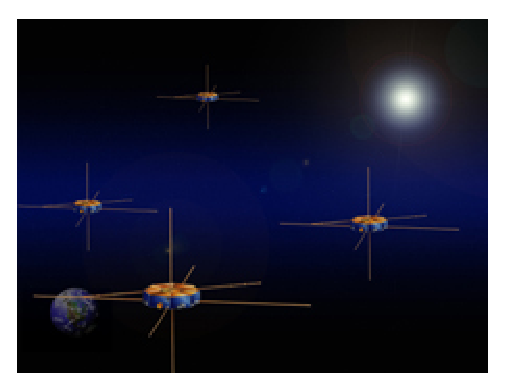
\psfig{file=figures/mms_spacecraft_formation.eps,height=1.2in}}
\caption{MMS Spacecraft Formation}
\label{fig:magneticfields}
\end{figure}

A reconnection event occurs when magnetic field lines cross allowing energetic particles to traverse from interstellar space into the Earth's magnetosphere releasing large quantities of heat and kinetic energy.  The diffusion region of a reconnection event starts on the day side magnetopause an quickly folds over to the Earth's magnetotail (Figure \ref{fig:magneticfields}).  This region is only 1-10 km in size but can travel at 10-100 km/hr \cite{swri} making it extremely difficult to measure.  Effects of a reconnection event are regularly experienced via the aurora borealis, interference with spacecraft GPS systems, and disruptions to electrical grids and communication networks.

\begin{figure}[H]
\centerline{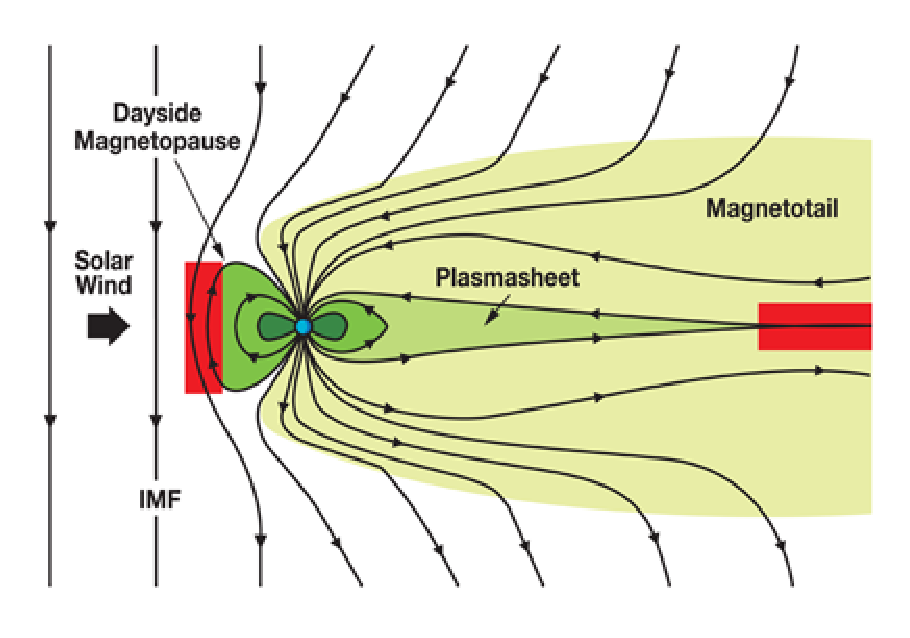
\psfig{file=figures/2d_earth_mag_field_lines.eps,height=1.2in}}
\caption{Earth's magnetic field}
\label{fig:magneticfields}
\end{figure}

Despite the widely experienced effects of reconnection events, very little about the microphysics inside its the diffusion region has been adequately measured.  Magnetometers, spectrometers, and other equipment currently in orbit are only able to capture a small fraction of the event's behavior.  Most equipment collect data from a single point or direction in space or some can get a 360 view of space by applying a slow spin to the spacecraft.  Both of these measurement methods are insufficient at capturing the structure of the diffusion region as it passes.

MMS's four satellites will be equipped with instrumentation mounted at the end of six boom extending out from the spacecraft's body along each major axis.  Four boom are the Spin Plane Double Probes (SDP) and two Axial Double Probes (ADP).  This configuration along with high resolution electron and ion spectrometers gives the constellation a new insight into the internal structure of the diffusion region.  The instrumentation at the ends of the boom are an advantage to the science portion of the mission, but create a unique challenge for the Attitude Determination and Control Systems (ADCS).  The satellites are spin stabilized at a rate of 3 rpm.  Disturbances to the rotation could translate into undesirable boom dynamics and nutations off the spin plane.



% Science questions to answer \cite{mms_website}
%     What determines when reconnection starts and how fast it proceeds?
%     What is the structure of the diffusion region?
%     How do the plasmas and magnetic fields disconnect and reconnect in the diffusion regions?
%     What role do the electrons play in facilitating reconnection?
%     What is the role of turbulence in the reconnection process?
%     How does reconnection lead to the acceleration of particles to high energies?


% \todo{image of formation flight}
% study microphysics of
%   magnetic reconnection
%   energetic particle acceleration
%   turbulence

% s/c MMS-1, MMS-2..MMS-4
% reconnection: Electromagnetic energy from the sun interacts with Earth's magnetosphere causing magnetic field lines to cross and create a burst of energy \cite{nasa_edge_video_ne_at_mms}
% magnetic reconnection measured ions and electrons as boundary passes to create 3d model of it passing by
% Fast plasma investigation
% probing the electron diffusion region (EDR) (passes too rapidly to get an accurate view with current equipment small (1-10 km) and rapidly moving (10-100 km/s))
% adjacent magnetic fields generally have significantly different orientations such that when they intersect, a large amount of energy is dispursed within a small region in the form of heat and kinetic energy.  The region = diffusion region
% explore magnetic reconnection
% dynamic regions of magnetosphere
% orbits planned to pass through the upstream and downstream magnetic reconnection sites
% 1) day side - solar wind field lines connection
% 2) down stream -
% 3) plasma travels down and causes the Arura
% through magnetospheric reconnection, portals allow energetic particles to traverse from outside to the interior of the magnetosphere
% predict when solar space weather within the magnetosphere and if they will affect orbiting satellites
% adverse space weather within the magnetosphere can negatively impact spacecraft system health GPS, induce disruptive current in electrical grids, communications, increased radiation exposure on trans-polar flights

% Difficult to understand
% magnetic boundary passes satellites quickly so has been hard to measure
% MMS has instruments to capture measurements
% Instruments mounted on all sides of the
% 8 sensors 1/30th sec instead of

% October 2014, Atlas five launch \cite{nasa_edge_video}

% Sensors
%   star sensor -> attitude
%   accelerometers -> $\Delta V$


% Fast Plasma Instrument (FPI) - controls
%   16 Dual Electron spectrometer (DES) Goddard built
%   16 Dual Ion Spectrometer (DIS) Japan *** built, hand delivered
%   180 degree and +- 22 degree measurement
%   30 millisec measurement rate 100x faster than previous missions entire view of sky
% FPI
%   despins data

% Instument Data processing Unit (IDPU) - brains of measurements
%   collects, compresses, transmits requested measurement data
%   configure while on mission

% booms
%   eight deployable booms
%   two 12.5m axial booms (electric field sensors)
%   four 60m wire booms
%   two 5m booms in spin plane for magnetometers
% rigid, wire, top/bottom booms
% important to keep consistent spin rate to get accurate estimates of boom location


% \section{Propulsion}

% types: solid propellents, bi propellents, electro propulsion, cold gas systems
% chose: mono-propellant blowdown - hydrozene power thrusters \cite{nasa_edge_video_propulsion}
% 3 rpm
% radial thrusters - spinning
% axial thrusters - prevent nutation

% concern:
% propulsion introduce distrubances

% 20 second pulses

% fuel limits by number of adjustments


% \section{performance requirements}

% $\pm 0.5$ deg attitude tollerance
% 1/10th of a second

\section{Research Objective}
\label{sec:ResearchObjective}

The work described in this thesis utilizes an experimental tabletop satellite (TableSat) \cite{vessthesis} to span three main efforts.  First is to create a physical model of a satellite from NASA's Magnetospheric MultiScale (MMS) Mission in order to validate and compare varied gyroless attitude determination and control (ADC) techniques.  The ADC systems must keep the TableSat rotating at a constant 3 rpm, prevent boom oscillations, and correct for detected nutations off the spin plane.  The second goal is to produce a software system that can be used to run against both theoretical simulations and experimental models.  The third goal is improve TableSat's use as an outreach tool.  The system should provide near ``real-time'' feedback of the system's state, allow for on-the-fly modification to control parameters, and be designed such that a individuals specializing in control systems could customize and extend its functionality without substantial computer science expertise.

\section{Past Work}
\label{sec:PastWork}

This work is a direct extension off of Vess' \cite{vessthesis} research using TableSat through Matlab Simulink and onboard flight controllers to demonstrate fundamentals of control theory.  The TableSat experimental design was modified to study the system dynamics of the instrument booms and nutation actuators in NASA's MMS mission satellites.  Previous experimental \cite{tsat1b} \cite{tsat1c} \cite{tsat2} and analytical \cite{mushawehthesis} ADC work at University of New Hampshire's Advanced Control Lab (ACL) has been done targeting the MMS mission.  The TableSat platform or similar derivations have also been adapted in investigate other areas of research including embedded systems development \cite{tablesat_xuml} and fault tolerant control \cite{tablesat_object_bench} \cite{nanjing_university}.


\section{Analytical and Experimental Testbed}
\label{sec:AnalyticalandExperimentalTestbed}



\section{Thesis Contributions}
\label{sec:ThesisContributions}

This research contributes to the field of feedback control, particularly as it relates to spin stabilized spacecraft, in the following ways:

\begin{itemize}
\item Gyroless observer-based controllers used to detect and eliminate nutations and maintain control of a spin stabilized satellite.
\item Improved capabilities of validating observer-based control methods by keeping identical control systems between analytical simulations and real experiments.
\item Allow clusters of estimators and controllers to all receive the same update for improved side-by-side comparisons of effectiveness.
\item Reduce time required to tune a controller by allowing for gain adjustments and swapping of estimation/control techniques on-the-fly.
\item Decompose quaternion state into separate rotational and nutation quaternions for use in error correction.
\item Use decomposed quaternion and differentiated rotational quaternions to decouple rate and attitude control.
\item Base quaternion state corrections on the representative rotational angle error, not the quaternion's sinusoidal scalar term.
\item Build the application such that the same control laws can be used to drive analytical simulations as well as experimental tests with physical systems.
\item Develop the application in a modular fashion to easily allow for future improvements and additions.
\item Control rates between modules such as sensors to estimators and estimators to controllers are independent and can operate at separate rates.
\item ``run-time'' feedback is available to visualize how the controller believes the system is responding.
\item A global clock instance is used for the authoritative time which during simulations can be adjusted in runtime to speed up or slow down the simulation to obtain better insight into the system dynamics.
\item Compensations for variable step sizes ($\delta t$) are made where able to protect the numerical integrity of the controller under large changes in control rates.
\item Code covered by proper software unit tests to validate and maintain expected behavior of the system during software upgrades.
\item Provide the combination of ``run-time'' visualizations and on-the-fly parameter/controller tuning for outreach programs.
\item Write the control application in a high level language to keep it accessible for improvements to control systems engineers with moderate programming experience.
\end{itemize}

\section{Thesis Outline}
\label{sec:ThesisOutline}



% %\include{notes/notes}
% %\include{appendices/appendices}

% %\include{appendices/bib}



% %\chapter{Equations}

% %\textbf{=============NOTES=============}
% %\include{equations/euler_body_rate}
% %\include{equations/quaternion_dynamics}
% %\include{equations/quaternion_body_rate}
% %\include{equations/quaternion_multiplication}
% %\include{equations/decompose_quaternion}
% %\include{quaternion/basics}
% %\textbf{=============NOTES=============}
% %\include{control/control_error}
% %\include{control/pid}

% %\include{Ch_TSat_Construction}

% % How is data aquired
% %\include{Ch_Data_aquisition}


% %Prior Versions - Matlab Code
% %\include{Ch_Prior_Versions}



% %Matlab Code
% %\include{Ch_Matlab_code}




% %Observer methods
% %\include{Ch_Observer_models}


% %\include{Ch_Controller_models}


% %\include{Ch_Observer_Control}


% %\chapter{Experimental Verification}
% %\label{chap:experimental}
% %\include{Ch_Experimental}



% %\chapter{Discussion of Results}
% %\label{chap:results}
% %\include{Ch_Results}

% %\chapter{Conclusions and Future Work}
% %\label{chap:conclusions}
% %\include{Ch_Conclustions}


% %\include{Appendix_Source_Code}
% %Matlab files
% %\chapter{Matlab Source Code}\label{ch:matlab_source}
% %\include{Matlab_Source_Code}

% \include{Bibliography}


% \newpage

% % \munfig{Credit: Southwest Research Institute}{mms_spacecraft_formation}{pretty/mms_spacecraft_formation.jpg}{0.4}

% % \munfig{Credit: http://earthobservatory.nasa.gov}{northern_lights_iss}{pretty/Northern-lights-ISS.jpg}{0.4}

% % \munfig{Credit: http://mms.gsfc.nasa.gov}{tetrahedron}{pretty/mms_dayside_tetrahedral_thumb.png}{0.4}

% % \munfig{Credit: http://mms.gsfc.nasa.gov}{2d_field_lines}{pretty/2d_earth_mag_field_lines.png}{0.4}
% % \munfig{Credit: http://mms.gsfc.nasa.gov}{instrument_deck_webview}{pretty/instrument_deck_webview.jpg}{0.4}
% % \munfig{Credit: http://mms.gsfc.nasa.gov}{observatory_dimensions1_webview}{pretty/observatory_dimensions1_webview.jpg}{0.4}
% % \munfig{Credit: http://mms.gsfc.nasa.gov}{observatory_interfaces_webview}{pretty/observatory_interfaces_webview.jpg}{0.4}
% % \munfig{Credit: http://mms.gsfc.nasa.gov}{observatory_webview}{pretty/observatory_webview.jpg}{0.4}

% % \munfig{Credits: ASRC Research and Technology/Barbara Lambert}{assembly}{pretty/713494main2_MMS-Observatory2-assembled-670.jpg}{0.4}

\end{document}